\documentclass{beamer}

\usetheme[progressbar=frametitle]{metropolis}
\usepackage{minted}
\usepackage{subfig}
\usepackage{hyperref}
\usepackage{multicol}

\title{How to Use Python and Mathematical Modeling to Better Understand the Impact of Electricity Pricing on Consumption}

\date{November 2, 2023}
\author{Saba Nejad}
\institute{PyData NYC 2023}

\begin{document}
\maketitle

\begin{frame}{Hi! I'm Saba. Thank you for coming to my talk.}
  \vspace{1cm}
  My name is Saba. I'm a Data Engineer at Point72. Today, I'll be walking you through part of my master's thesis that I worked on and defended two years ago at MIT.
  \newline
  \newline
  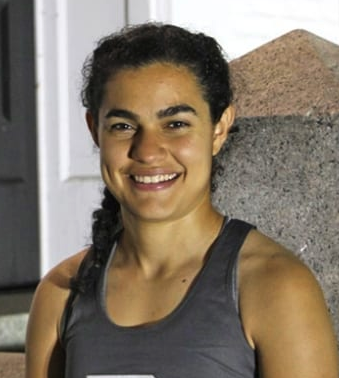
\includegraphics[width=0.2\textwidth]{images/saba-nejad.png}
\end{frame}

\begin{frame}{Goals for this talk}
  % If you walk away with anything today, I want it to be the following two points.
  \begin{itemize}
  \item<+-> Before starting to analyze your data, you should know details about your data:
    \begin{itemize}
      \item how it was collected
      \item its biases
      \item dimenstionality, fill-rate, etc.
    \end{itemize}
  \item<+-> Before trying to fit a model to your data, you should have a mathematical model rooted in the real world.
  \end{itemize}
\end{frame}

\begin{frame}{What are we going to talk about?}
  To that end, I'll be talking about,
  % I will walk you through a specific data modeling problem on a specific dataset, the techniques I used and found helpful and I hope you'll find them helpful too.
  \begin{itemize}
    \item<+-> the data from a trial in London that implemented a particular pricing model on a subset of houses to quantify the impact of pricing on electricity consumption.
    \item<+-> the steps I took to understand this data, and methods I used to prep, clean, and process the data.
    \item<+-> the thinking behind the mathematical framing of the problem.
    \item<+-> the analysis based on the particular dataset and mathematical model.
    \item<+-> results, takeaways, lessons learned.
  \end{itemize}
\end{frame}

% \begin{frame}{Overview of the Talk}
%   \begin{itemize}
%   \item<+-> Introduce the Problem Space; Define Terminology
%   \item<+-> Introduce the Trial and the Dataset
%   \item<+-> Mathematical Model
%   \item<+-> Data Prep, Cleaning, Processing
%   \item<+-> Results, Takeaways, Conclusion
%   \end{itemize}
% \end{frame}

\section{Useful Details about the Problem Space}
% Here, we will walk through the specifc details within electricity pricing that will help with understanding the general problem

\begin{frame}{In electicity, there is a supply and demand constaint.}
  \begin{itemize}
    \item<+-> Electricity is unique in that its \textbf{storage is prohibitively costly}.
    \item<+-> As a result, \textbf{supply must meet demand} at all times. 
    \item<+-> If demand exceeds supply, there will be a power outage. 
    \item<+-> Power outages are extremely costly and we try to prevent them as much as possible.
  \end{itemize}
\end{frame}

\begin{frame}{Demand Response is a tool that helps lower demand.}
  \begin{itemize}
    \item<+-> This unique feature of electricity, poses a \textbf{challenge}. 
    \item<+-> Imagine an unpredictably hot day where there is more demand than expected.
    \item<+-> To prevent a power outage, we need close to real-time methods to lower demand.
    \item<+-> \textbf{Demand Response} is one such method.
  \end{itemize}
\end{frame}

\begin{frame}{Demand Response visual example}
  \centering
  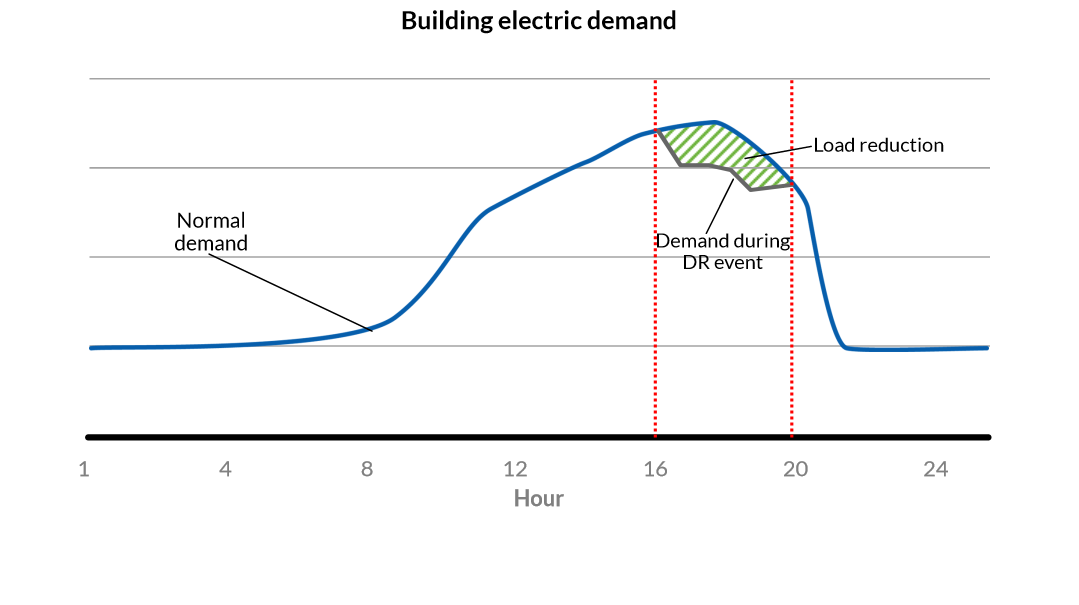
\includegraphics[width=0.85\textwidth]{images/demand-response.png}
\end{frame}

\begin{frame}{One demand response method are blast texts.}
  \centering
  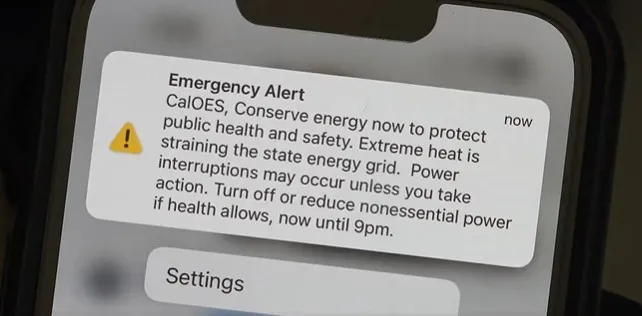
\includegraphics[width=0.8\textwidth]{images/OES-power-text.png}
\end{frame}

\begin{frame}{Another demand response method is using pricing models.}
  These pricing models \textbf{increase} price, to incentivize people to 
  \begin{itemize}
    \item<+-> Assumption 1: Demand can be shifted around.
    \item<+-> Assumption 2: Consumers are price sensitive i.e. they will respond to price incentives.
    \item<+-> Two pricing models:
    \begin{itemize}
      \item<+-> Time of Use Pricing (ToU)
      \item<+-> Dynamic Time of Use Pricing (dToU)
    \end{itemize}
  \end{itemize}
\end{frame}

\begin{frame}{Repeat}
  There is a pricing model, called \textbf{Dynamic Time of Use Pricing}, that uses price incentives to lower demand on the grid and prevent a power outage.
\end{frame}

% implicit in this pricing model is that there's correlation between demand and price. the idea is that we will respond to the incentive because
% we're price sensitive beings. but the question is can the pricing model *cause* us to lower our consumption. in the next section, we'll walk through 
% some mathematical tools to investigate and qualify the causal link between the pricing model and consumption.

\begin{frame}{Understanding causality and some useful terminology}
  \begin{itemize}
    \item<+-> What is a treatment? What is the treatment effect?
    \item<+-> What is a `unit' undergoing treatment?
    \item<+-> What does it mean for something to have a causal effect on something else?
    % need not be an actual treamment, the thing or intervention whose impact we are trying to study
    \item<+-> What is the counterfactual?
  \end{itemize}
    \centering
    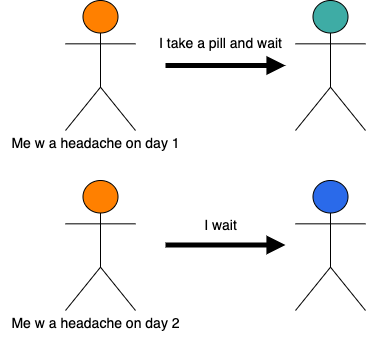
\includegraphics[width=0.5\textwidth]{images/headache-treatment-effect.png}
\end{frame}

\begin{frame}{The Fundamental Problem of Causal Inference (FPCI)}
  \begin{itemize}
    \item<+-> Assume $X \in\{0,1\}$ is a binary causal variable and $Y$ is a response variable (which may be continuous).
    \item<+-> Assume $X$ has a causal effect on $Y$.
    \begin{itemize}
      \item $Y_0$ := the value of $Y$ when $X=0$ (untreated unit)
      \item $Y_1$ := the value of $Y$ when $X=1$ (treated unit)
      \item $T = Y_1 - Y_0$ := the treatment effect
    \end{itemize}
    \item<+-> $Y_0$ and $Y_1$ are \textbf{counterfactuals} of one another. We observe \textbf{only} $Y_1$ or $Y_0$, but not both at the same time.
    % the reason counterfactuals are estimated are SO WE CAN ESIMATE THE TREATMENT EFFECT
  \end{itemize}
\end{frame}

\begin{frame}{Solutions Around FPCI}
  \begin{enumerate}
    \item<+-> Temporal Stability \& Causal Transience
    % \begin{enumerate}
    %   \item<+-> the causal effect of $X$ on $Y$ is the same at every point in time
    %   \item<+-> and the causal effect of $X$ on $Y$ is reversible (so having once been exposed $X$ doesn't permanently change the effect of $X$ on $Y$)
    %   \item<+-> applies in lab settings, water molecules, for example. doesn't apply to humans
    % \end{enumerate}
    \item<+-> Unit Homogeneity
    % \begin{enumerate}
    %   \item<+-> response variables are identical for all units
    %   \item<+-> applies in lab settings, water molecules, for example. doesn't apply to humans
    % \end{enumerate}
    \item<+-> Estimate causal effects for populations rather than units
    % \begin{enumerate}
    %   \item<+-> applies to populations of humans, and this problem!
    % \end{enumerate}
  \end{enumerate}
\end{frame}

\begin{frame}{Solutions Around FPCI for this Trial}
  \begin{enumerate}
    \item Temporal Stability \& Causal Transience {\color{red}{X}}
    \item Unit Homogeneity {\color{red}{X}}
    \item Estimate causal effects for populations rather than units {\color{green}{\checkmark}}
  \end{enumerate}
\end{frame}

\begin{frame}{Random samples of populations are studied to estimate treatment effects.}
  \begin{itemize}
    \item<+-> It's difficult to estimate the treatment effect for a unit. \\
    \indent $\implies$ FPCI makes it \textbf{necessary} to study a \textbf{population vs a unit}. The \textbf{larger the population}, the easier to robustly estimate treatment effects.
    \item<+-> When estimating treatment effect for populations, to remove bias terms, we want groups that behave similarly out of sample. \\
    \indent $\implies$ analyses are done on \textbf{random samples} of populations.
  \end{itemize}
\end{frame}

\begin{frame}{What have we learned and where are we headed?}
  in summary, we want large, random samples of populations to estimate effect of a treatment.
  perhaps connecting this back to the second lesson of the talk, its important to base your analysis in some mathematical framework because it'll change what you are able to do with the data you have.
  now we have some mathematical tools in our toolbox to study causality and estimate treatment effects.we know a bit about the 
  pricing model in this trial. now let's go learn more about the trial and the data
\end{frame}

\section{The Details of the Trial Studied}

\begin{frame}{High Level Overview of the Trial}
  \centering
  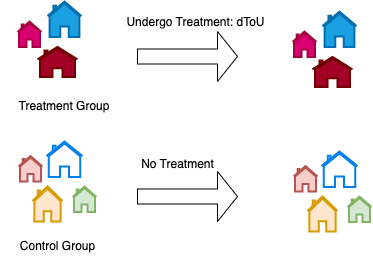
\includegraphics[width=0.5\textwidth]{images/trial-high-level.png}
\end{frame}

\begin{frame}{Low Carbon London Smart Meter Trial}
  \begin{itemize}
    \item<+-> Motivation: The Climate Change Act of 2008 sets the target of reducing carbon emissions to 20\% of 1990 levels by 2050.
    \item<+-> Data spans November 2011 and February 2014.
    \item<+-> Treatment took place in the calendar year 2013.
    \item<+-> Readings were taken at half hourly intervals, for the entire duration of the trial, and for 5600 houses in total (around 167M records).
  \end{itemize}
\end{frame}

\begin{frame}{dToU: pre-set prices, implemented at different times of day}
  \begin{itemize}
    \item<+-> dToU price bands vs static pricing model:
    \begin{table}[]
      \vspace{0.2cm}
      \centering
      \begin{tabular}{|l|l|}
        \hline
        dToU Pricing Model & Static Pricing Model \\ \hline
        High (67.20 p/kWh) & 14.228 p/kWh \\ \hline
        Normal (11.76 p/kWh) & 14.228 p/kWh \\ \hline
        Low (3.99 p/kWh) & 14.228 p/kWh \\ \hline
      \end{tabular}
    \end{table}
  \end{itemize}
\end{frame}

\begin{frame}{dToU: pre-set prices, implemented at different times of day}
  \begin{itemize}
    \item<+-> ``Dynamic": Times of day when households would be subject to high price point was communicated a day ahead via the Smart Meter In Home Display or text message.
    \vspace{0.3cm}
    \begin{center}
    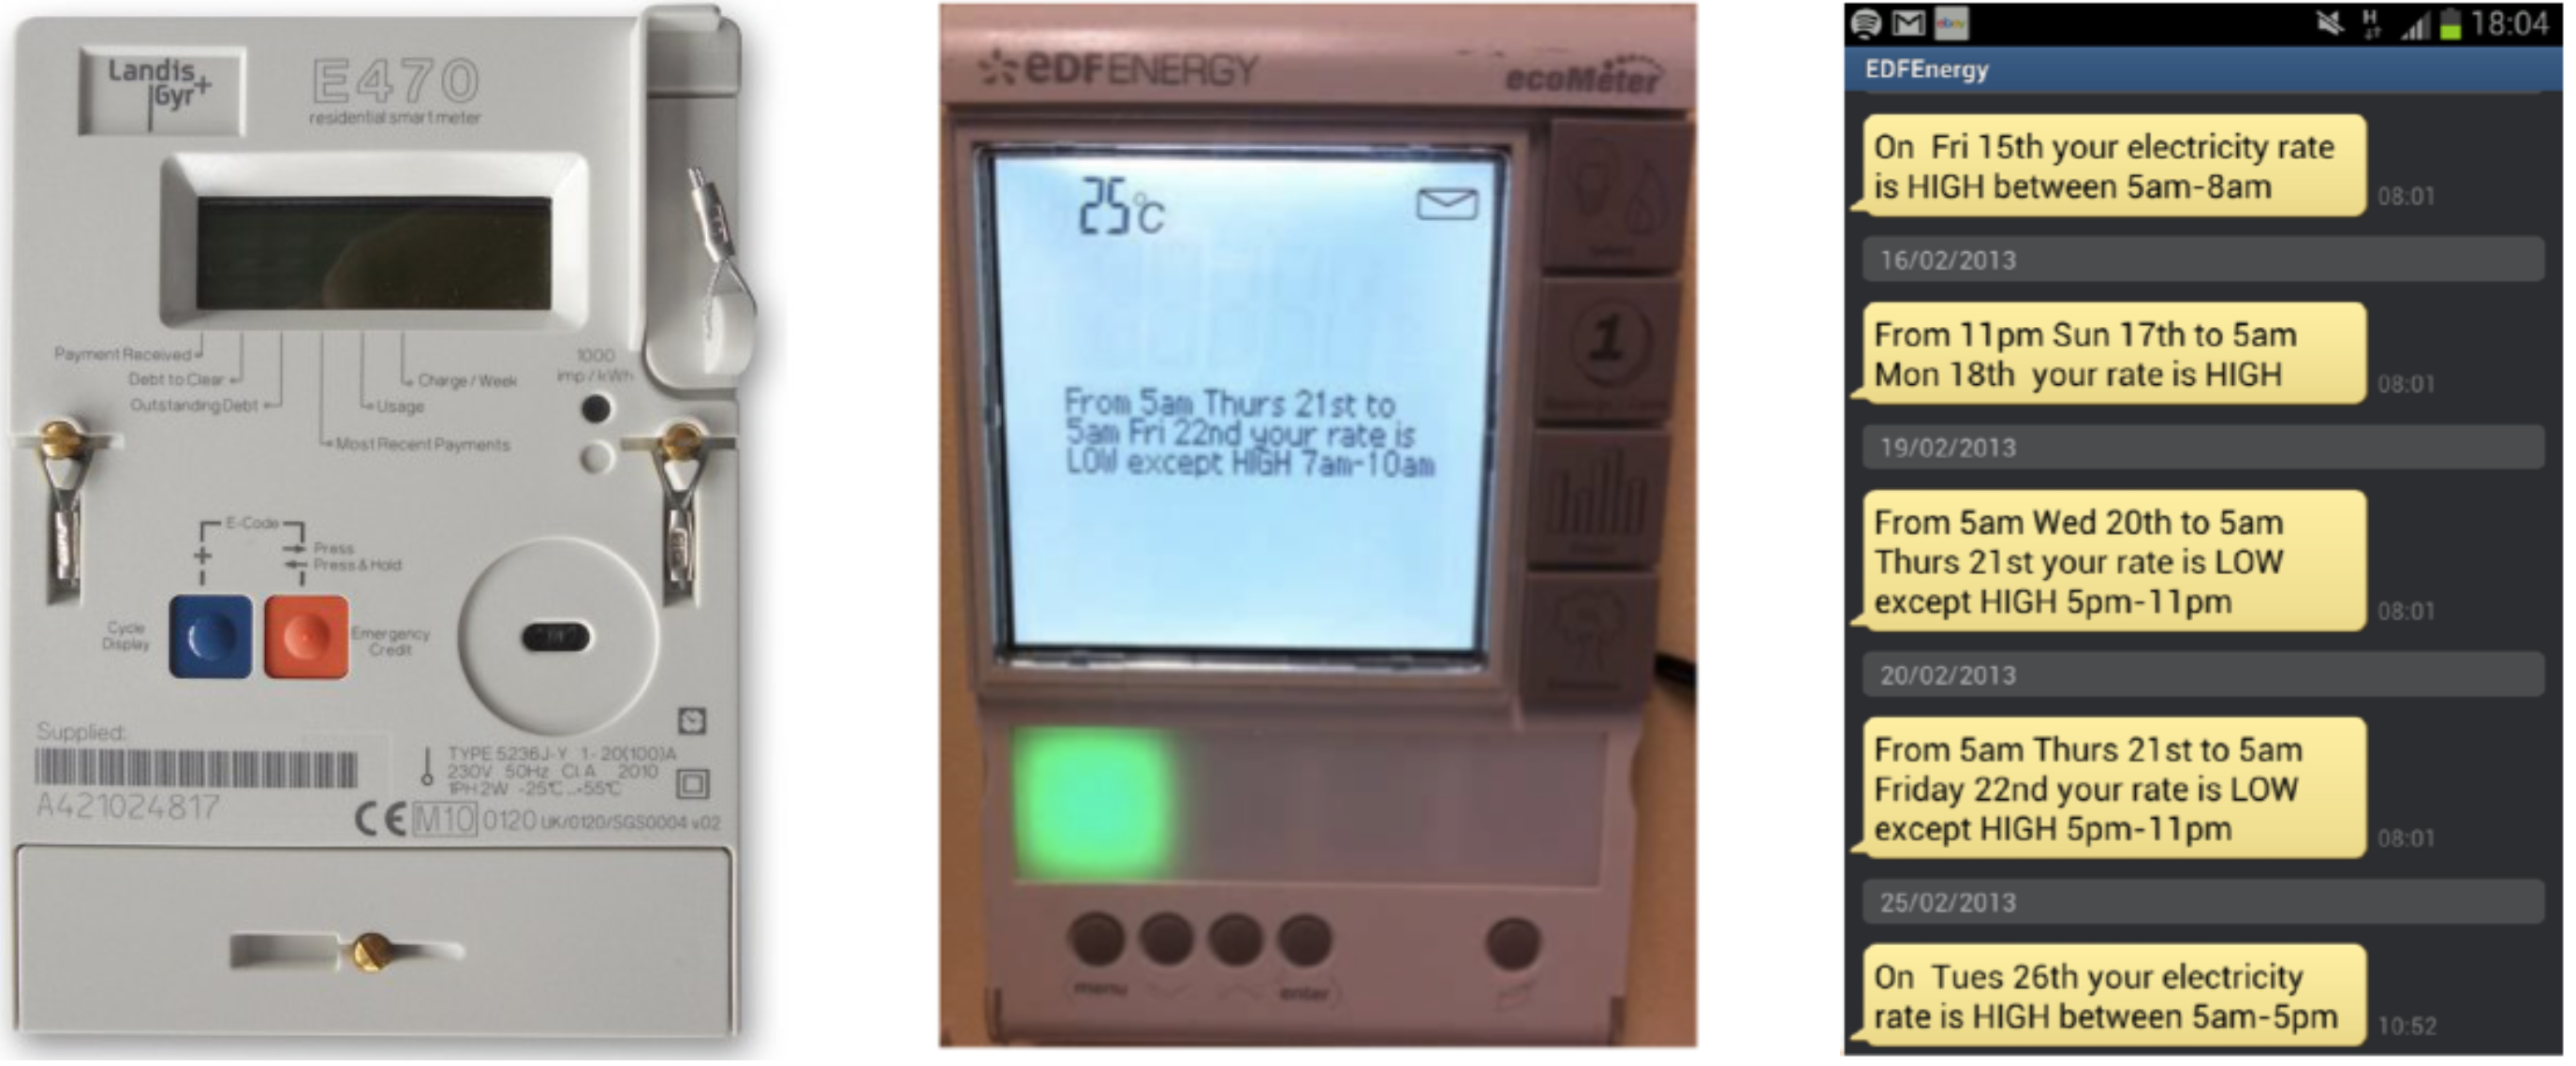
\includegraphics[width=0.87\textwidth]{images/day-ahead-pricing.png}
    \end{center}
  \end{itemize}
\end{frame}

% \begin{frame}{Additional Features: Discrete Socio-Economic Categories}
%   % discrete socio-economic feature per household included in the data
%   % \begin{figure}
%   %   \centering
%   %   \subfloat{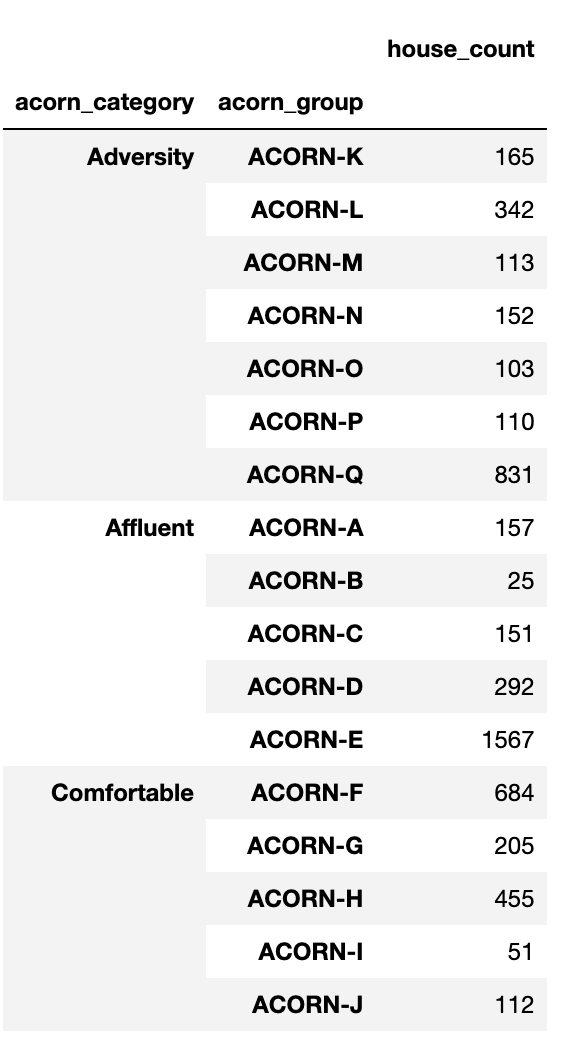
\includegraphics[width=5cm]{images/acorn-group-levels.png}}
%   %   \qquad
%   %   \subfloat{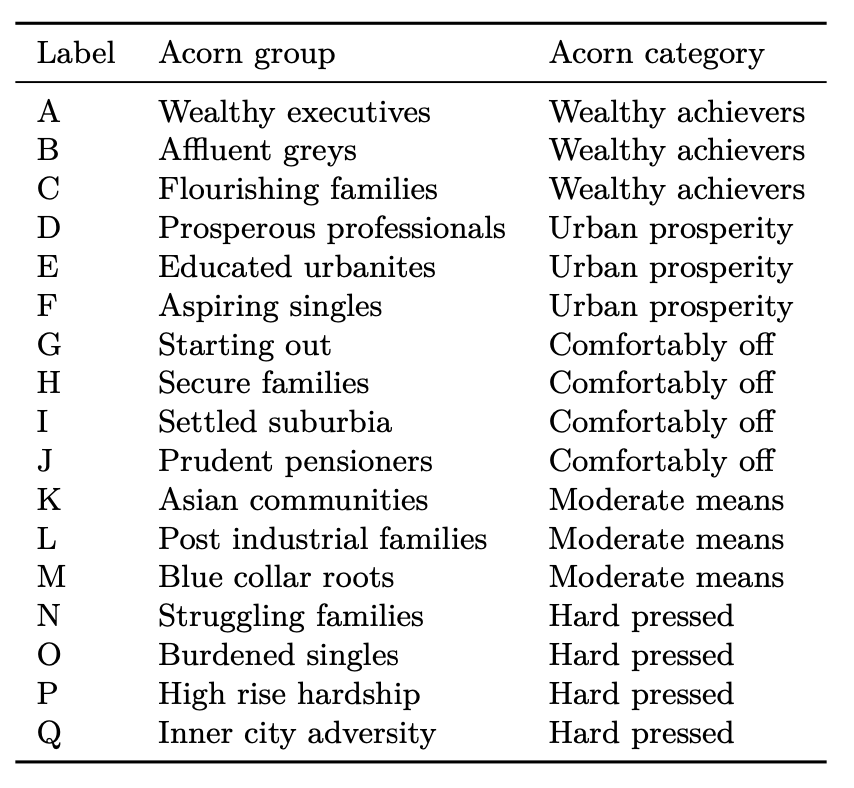
\includegraphics[width=5cm]{images/acorn-groups.png}}
%   % \end{figure}
%   % \begin{figure}[] 
%   %   \centering
%   %   \subfloat[]{
%   %       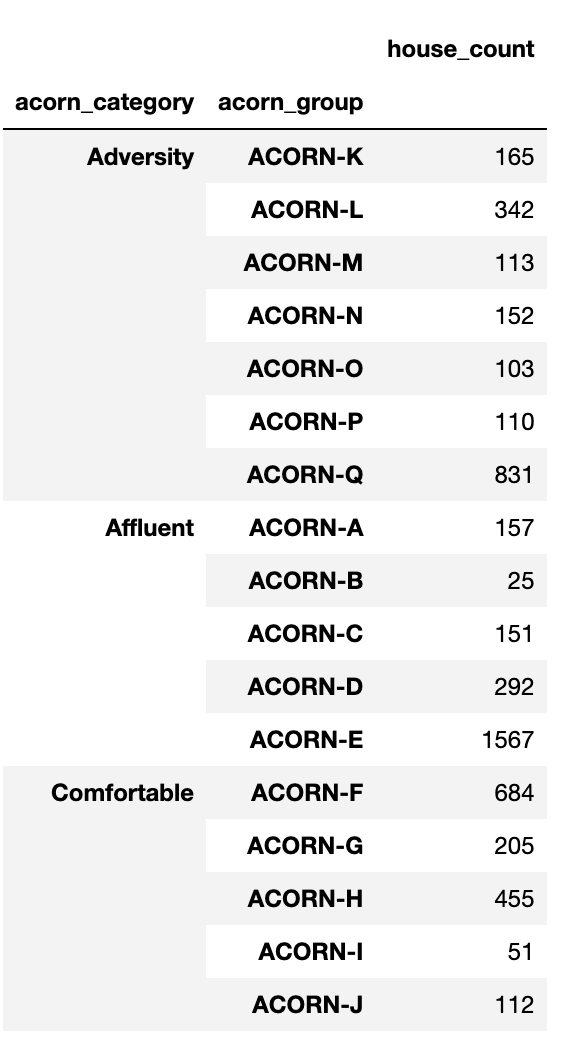
\includegraphics[width=0.4\textwidth]{images/acorn-group-levels.png}
%   %       }
%   %   \hfill
%   %   \subfloat[data b]{
%   %       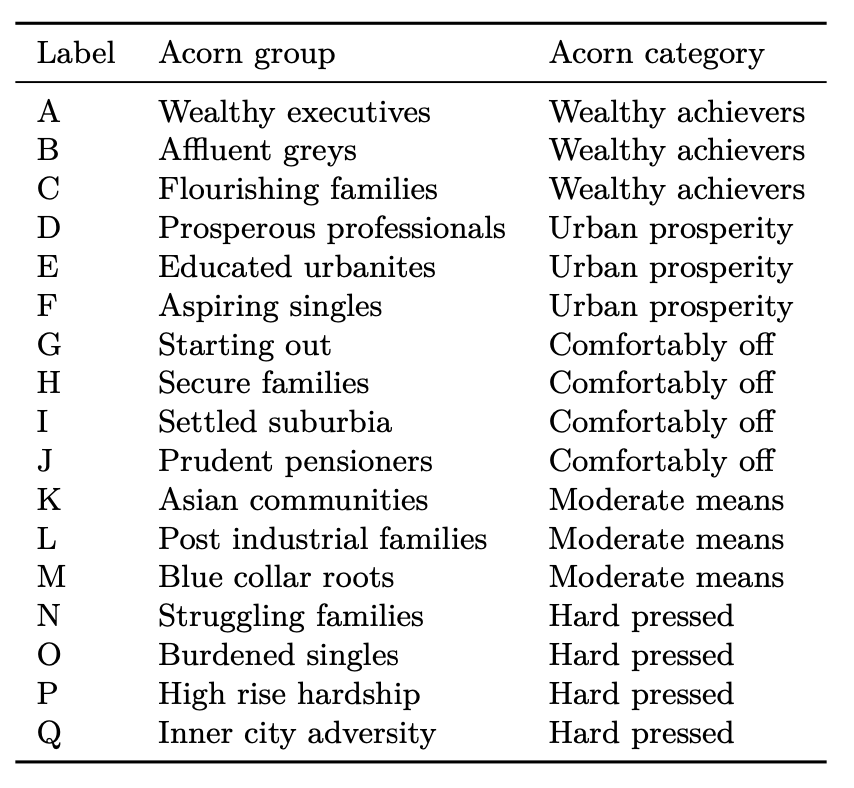
\includegraphics[width=0.4\textwidth]{images/acorn-groups.png}
%   %       }
%   % \end{figure}
% \end{frame}

\begin{frame}{Features: Two Levels of Discrete Socio-Economic Categories}
  \centering
  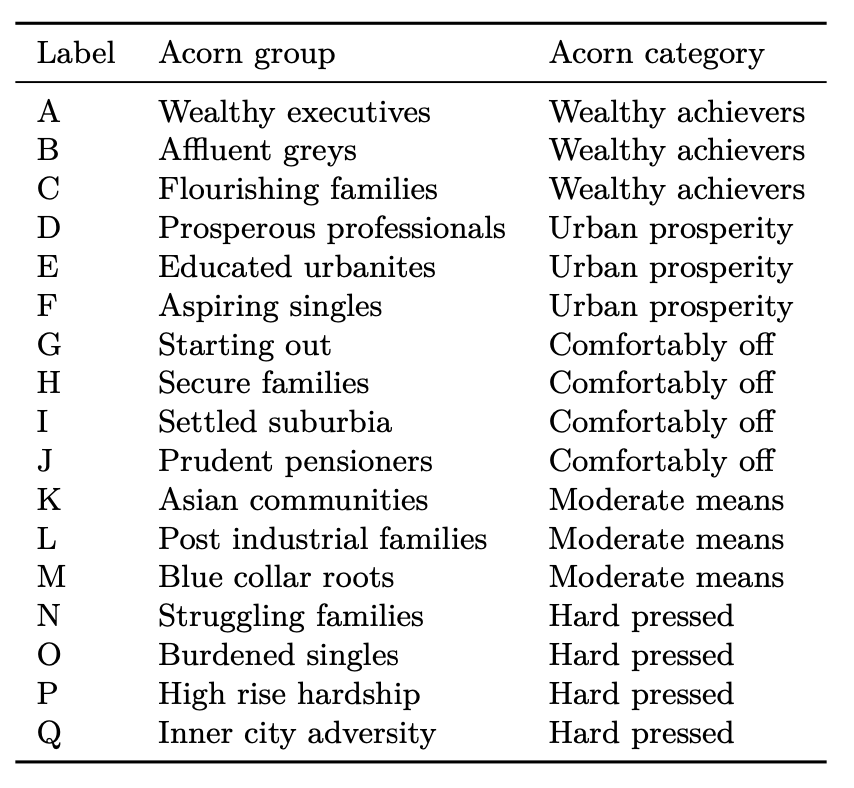
\includegraphics[width=0.65\textwidth]{images/acorn-groups.png}
\end{frame}

% \begin{frame}{Additional Features: Discrete Socio-Economic Categories}
%   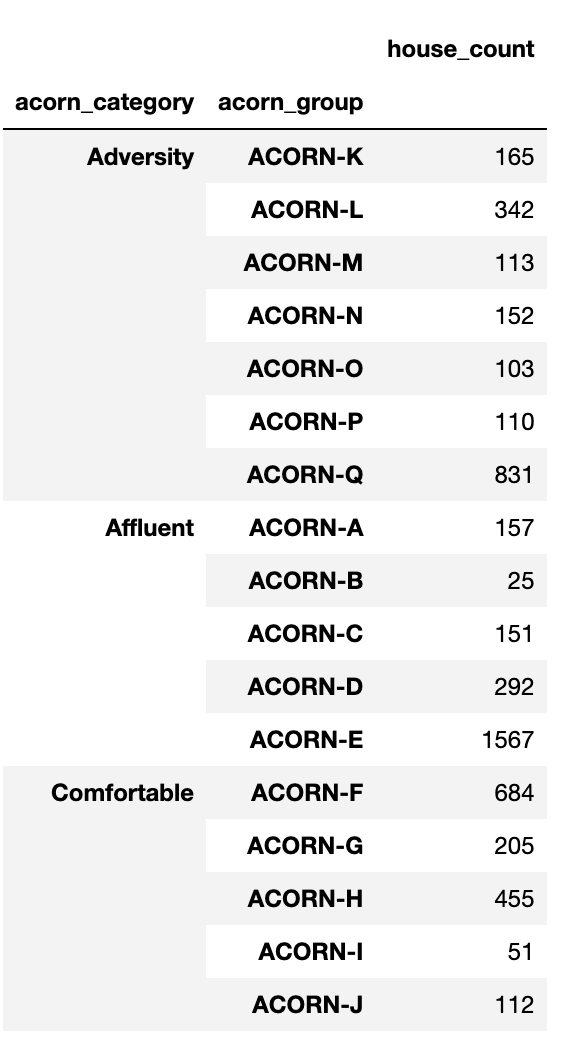
\includegraphics[width=1\textwidth]{images/acorn-group-levels.png}
% \end{frame}

\begin{frame}{Features: Two Levels of Discrete Socio-Economic Categories}
  \centering
  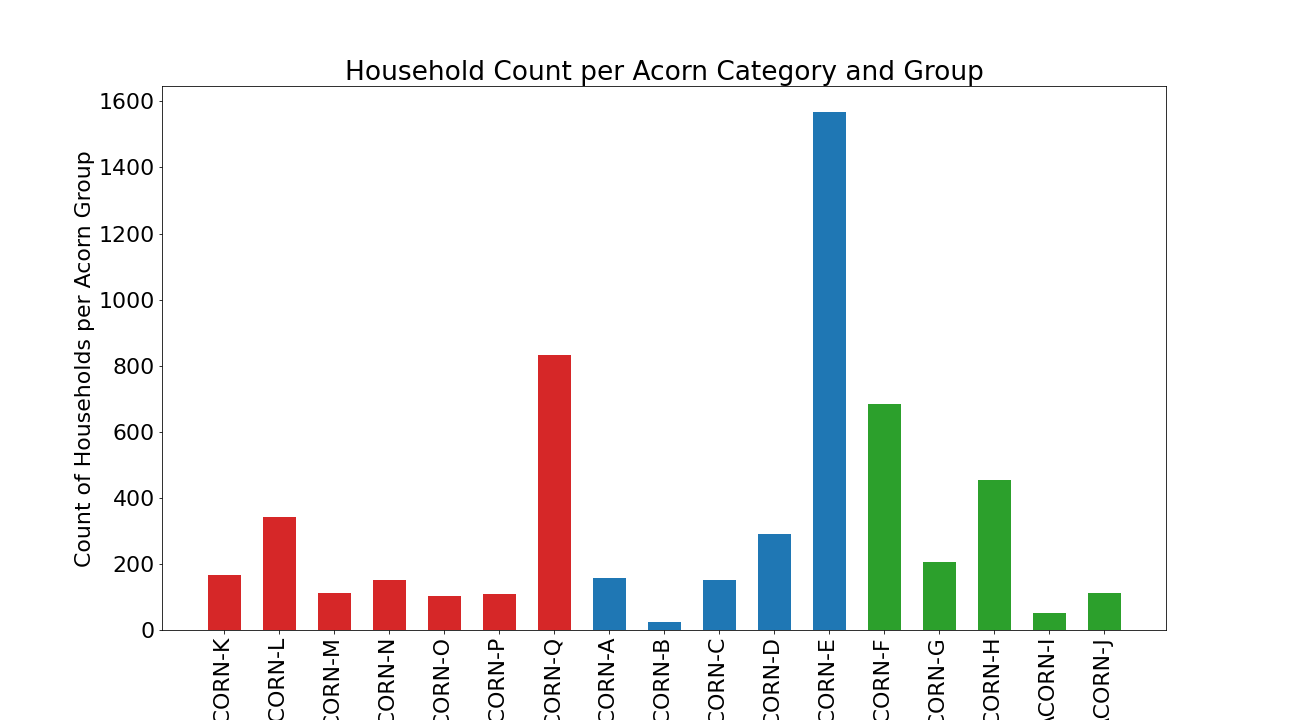
\includegraphics[width=0.8\textwidth]{images/acorn-group-category-house-count.png}
\end{frame}

\begin{frame}{Biases I: Treatment group opted in.}
  \textbf{The trial is double opt-in}:
  \begin{enumerate}
    \item<+-> Households opt into sharing their data with the trial at all.
    \item<+-> Some opted into undergoing dToU pricing in 2013.
  \end{enumerate}
\end{frame}

\begin{frame}{Biases II: There were cash incentives for the treatment group.}
  The treatment group was given some incentives: 
  \begin{itemize}
    \item A guarantee that they will be reimbursed at the end of trial if they are worse off on the dToU tariff than they would have been on their previous tariff.
    \item Assurances regarding how many hours would be charged at the high price band.
    \item \textsterling100 for signing up to the dToU tariff.
    \item Another \textsterling50 for staying on the dToU tariff until the end of trial.
    \item Entry into a prize draw after completion of the post trial survey.
  \end{itemize}
\end{frame}

\begin{frame}{The two groups were not biased geographically}
  \begin{figure}
    \centering
      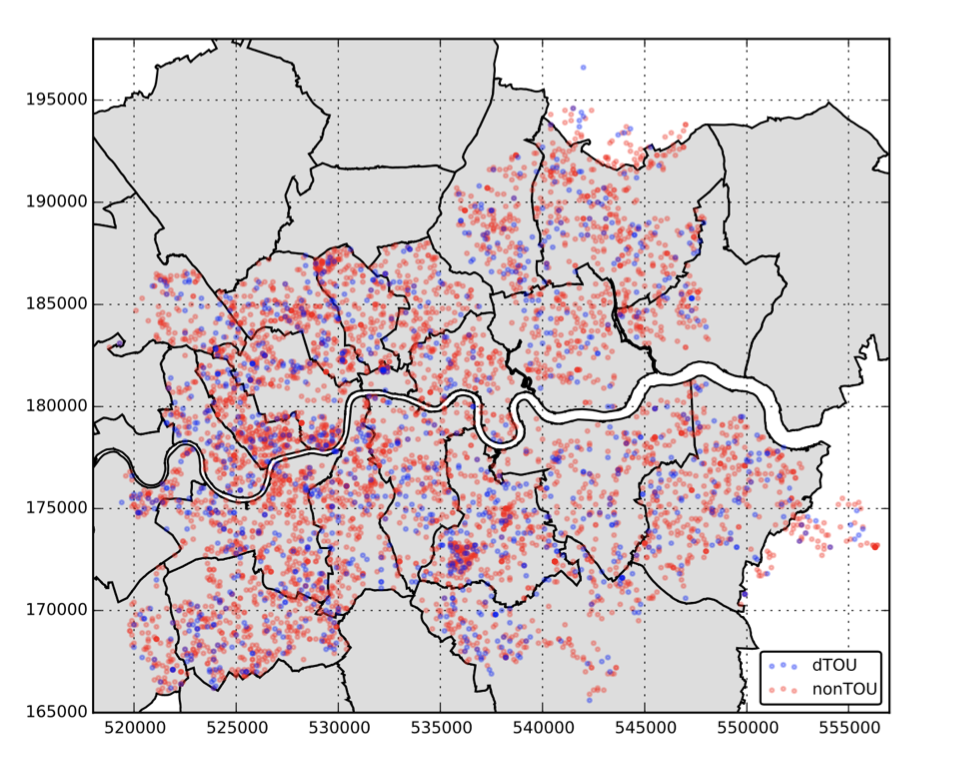
\includegraphics[width=0.7\textwidth]{images/london-geo-breakdown.png}
      \caption{Trial household sample locations overlaid on the borough boundary map of Greater London. This shows that the treatment and control group were representative samples of Greater London.}
  \end{figure}
\end{frame}

\begin{frame}{The two groups were not biased socio-economically}
  \begin{figure}
    \centering
    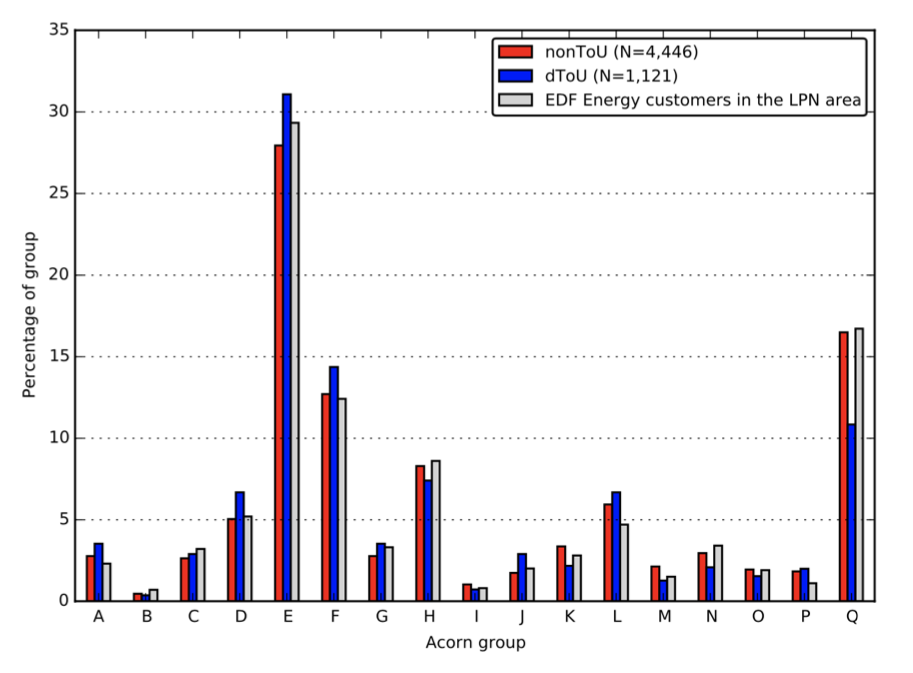
\includegraphics[width=0.85\textwidth]{images/london-socio-breakdown.png}
    \caption{The treatment and control groups were also representative socio-economic samples of Greater London.}
  \end{figure}
\end{frame}

\begin{frame}{Onboarding households creates a missing data issue.}
  \begin{itemize}
    \item 2012: Users were still onboarding.
    \item 2013: Some users dropped out of both the treatment and the control groups
    \item \texttildelow5,600 total households participated: \texttildelow4,500 were in the control group, \texttildelow1,100 were in the treatment group.
  \end{itemize}
  \vspace{-0.25cm}
  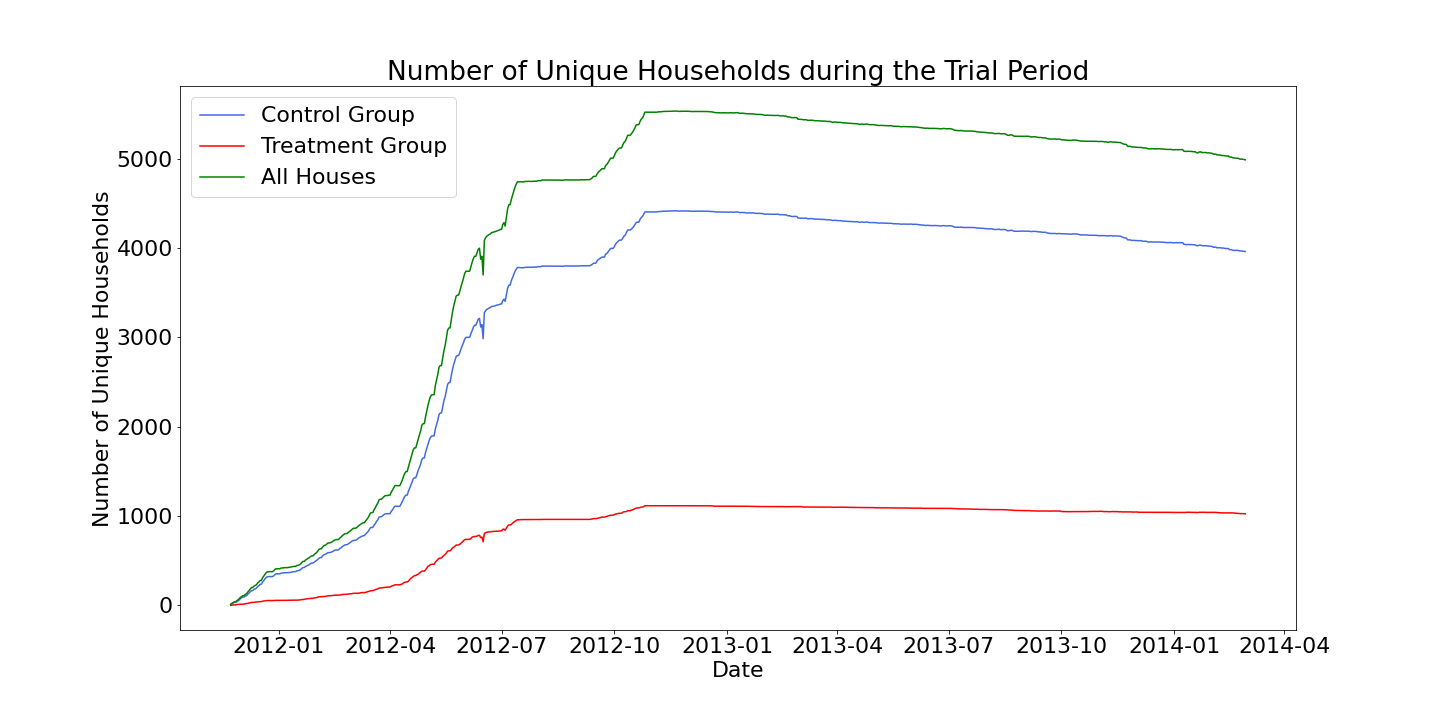
\includegraphics[width=1\textwidth]{images/house-count.png}
\end{frame}

\begin{frame}{Treatment vs Control Group Baselines}
  \begin{itemize}
    \item<+-> Though our groups are \textbf{geographically and socio-economically balanced}, one group opted into dToU pricing and was offered some incentives.
    \item<+-> What are some reasons the baselines might differ given what we know?
    \begin{itemize}
      \item<+-> price sensitive group opted in
      \item<+-> low consuming group opted in
      \item<+-> those households are flexible time-wise: particular jobs, hours, etc.\
    \end{itemize}
  \end{itemize}
\end{frame}

\section{Let's formulate the mathematical model that will inform our analysis.}

\begin{frame}{Let's establish some symbology standards}
  Consider the following segmentation of the data.
  \begin{itemize}
    \item $\alpha_y$ := control group's consumption matrix during year $y$
    \item $\beta_y$ := treatment group's consumption matrix during year $y$
  \end{itemize}
\end{frame}

\begin{frame}{What are these matrics and what is in them?}
  \begin{multicols}{2}
  $$
  \alpha_y = \left[\begin{array}{cccc}
  a_{11} & a_{12} & \cdots & a_{1 n_c} \\
  a_{21} & a_{22} & \cdots & a_{2 n_c} \\
  \vdots & \vdots & \ddots & \vdots \\
  a_{t 1} & a_{t 2} & \cdots & a_{t n_c}
  \end{array}\right]
  $$
  \break
  $$
  \beta_y = \left[\begin{array}{cccc}
  b_{11} & b_{12} & \cdots & b_{1 n_t} \\
  b_{21} & b_{22} & \cdots & b_{2 n_t} \\
  \vdots & \vdots & \ddots & \vdots \\
  b_{t 1} & b_{t 2} & \cdots & b_{t n_t}
  \end{array}\right]
  $$
  \end{multicols}
  \begin{itemize}
  \item[]<+-> $\alpha$ matrics are of size $\alpha_{t \times n_c}$; $\beta$ matrics are of size $\beta_{t \times n_t}$.
  \item[]<+-> $t$ is the number of half-hour measurements in a year ($t = 365 \times 48 = 17,520$ for 2012 and 2013).
  \item[]<+-> $n_c$ is the number of households in the control group; $n_t$ is the number of households in the treatment group. 
  \end{itemize}
\end{frame}

\begin{frame}{Our goal is to find a good estimate for the counterfactual consumption.}
  % \begin{table}[h!]
  % \centering
  %   \begin{tabular}{|p{3cm}|p{3.5cm}|p{3.5cm}|}
  %       \hline
  %       Year & Control Group & Treatment Group \\
  %       \hline
  %       2011 & $\alpha_{2011}$ & $\beta_{2011}$ \\
  %       2012 & $\alpha_{2012}$ & $\beta_{2012}$ \\
  %       2013 & $\alpha_{2013}$ & $\hat\beta_{2013}$ \\
  %       2014 & $\alpha_{2014}$ & $\beta_{2014}$ \\
  %       \hline
  %   \end{tabular}
  % \end{table}
  \begin{itemize}
    \item[]<+-> $\hat\beta_{2013}$ is the counterfactual consumption for $\beta_{2013}$.
    \item[]<+-> $T = \hat\beta_{2013} - \beta_{2013}$ is the treatment effect.
    \item[]<+-> Goal is to \textbf{find a good estimate} for $\hat\beta_{2013}$.
  \end{itemize}
\end{frame}

\begin{frame}{Naive Model: Use Treatment Group in 2013 as Counterfactual}
  If we didn't know about all these biases, we \textit{could} use control group in 2013 as the counterfactual estimate for treatment group in 2013.
  \begin{align}
    \begin{split}
      \hat\beta_{2013} & \approx \alpha_{2013} \\
      T & = \beta_{2013} - \hat\beta_{2013} \\
        & = \beta_{2013} - \alpha_{2013}
    \end{split}
  \end{align}
\end{frame}

\begin{frame}{Treatment vs Control Group Baselines}
  \centering
  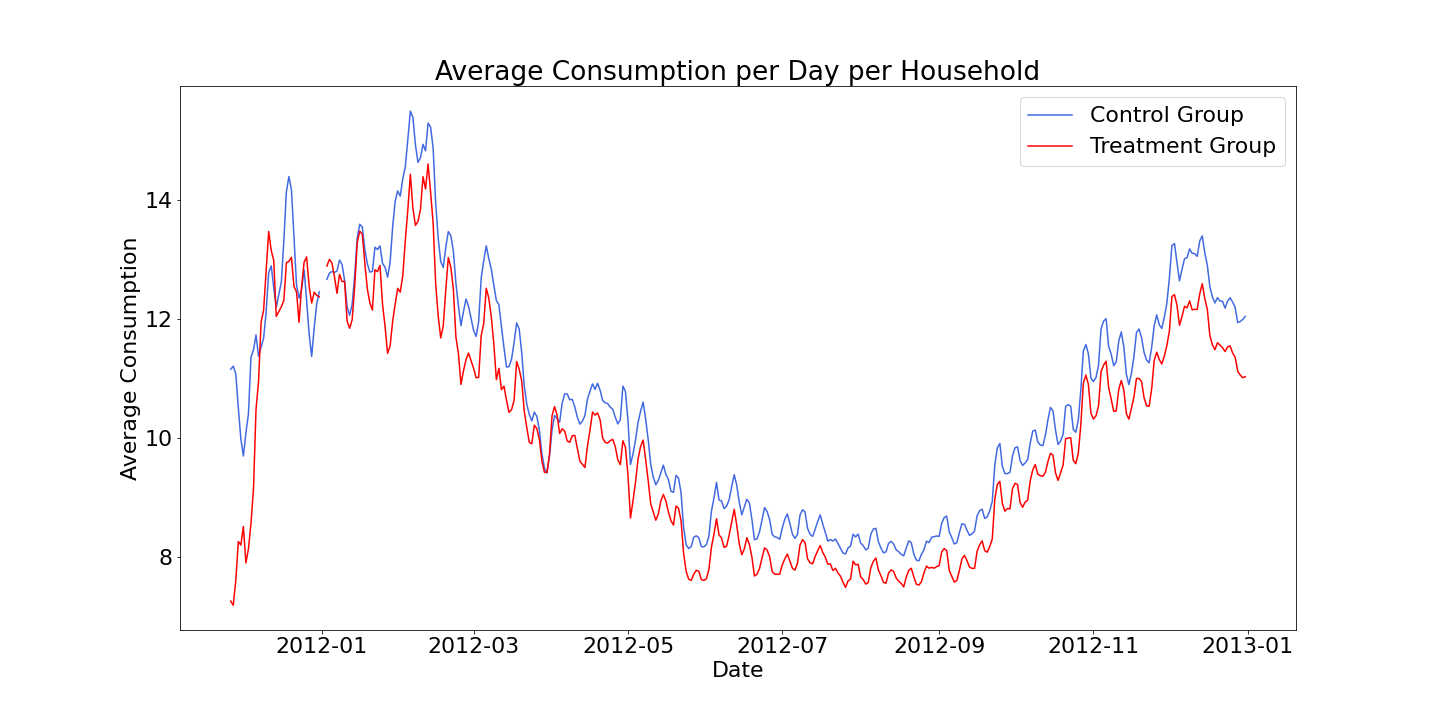
\includegraphics[width=1\textwidth]{images/avg-consumption-per-day-baseline.png}
  $\implies$ the two groups don't have the same baseline electricity consumption patterns.
\end{frame}

\begin{frame}{Sophisticated Naive Model}
  Let's instead use treatment group in 2012 as the counterfactual estimate for treatment group in 2013.
  \begin{align}
    \begin{split}
      \hat\beta_{2013} & \approx \beta_{2012} \\
      T & = \beta_{2013} - \hat\beta_{2013} \\
        & = \beta_{2013} - \beta_{2012}
    \end{split}
  \end{align}
\end{frame}

\begin{frame}{Changes from Time: 2012 vs 2013}
  \centering
  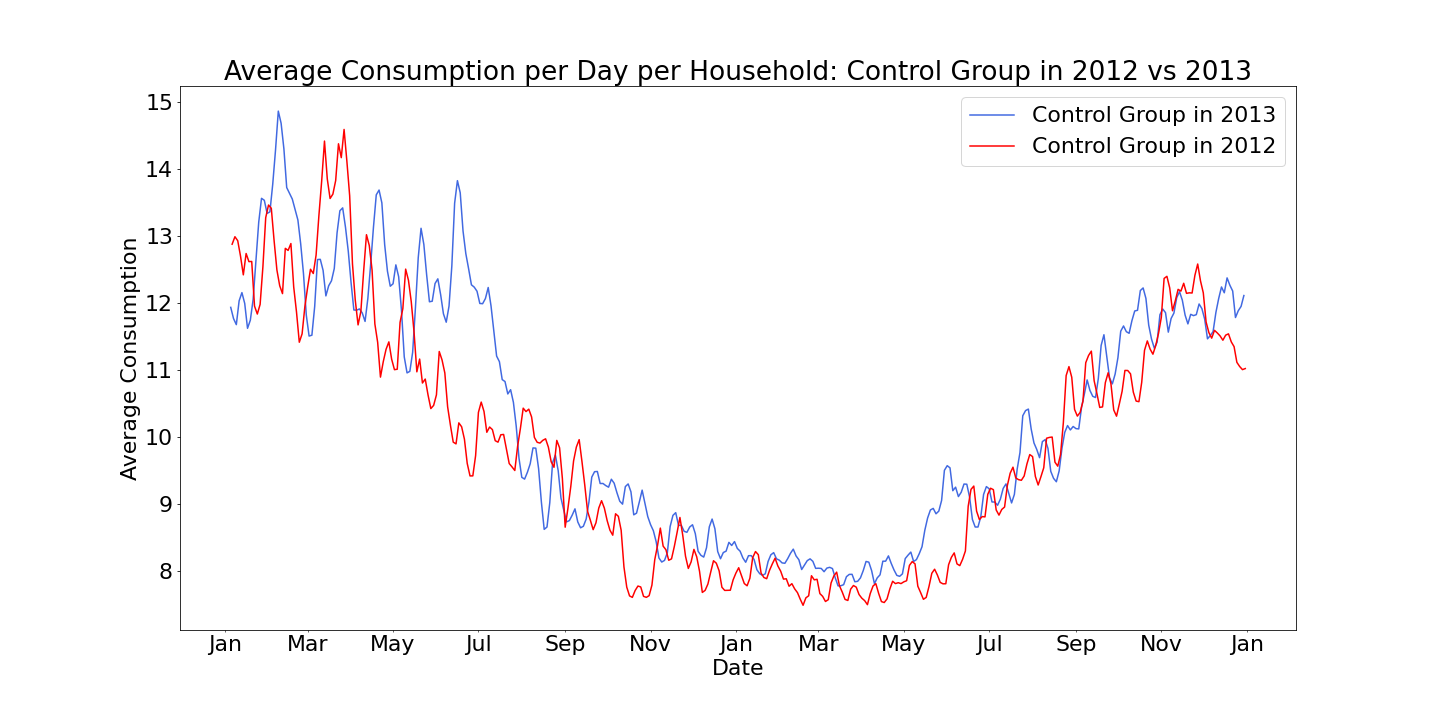
\includegraphics[width=1\textwidth]{images/yoy-changes-control-group.png}
  $\implies$ Things changed between the two years even for the control group.
\end{frame}

\begin{frame}{Treatment vs Control Group Baselines}
  \centering
  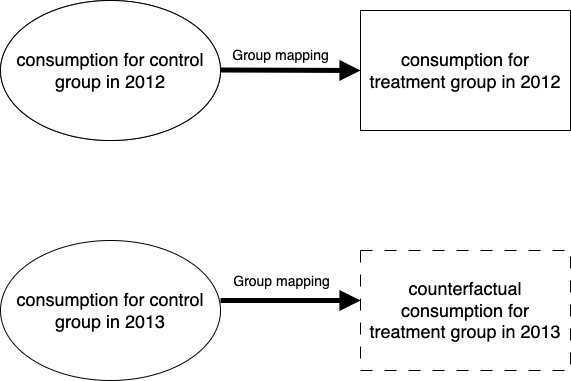
\includegraphics[width=0.8\textwidth]{images/group-mapping.png}
\end{frame}

\begin{frame}{Treatment vs Control Group Baselines}
  \centering
  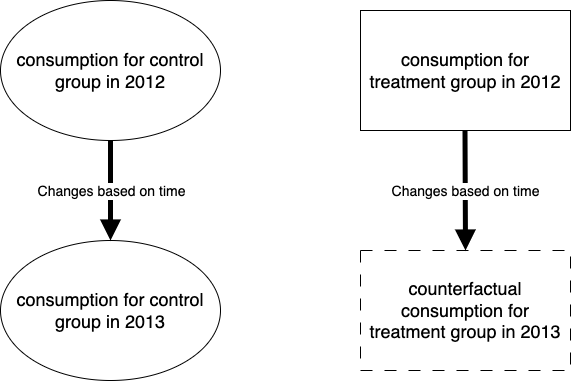
\includegraphics[width=0.8\textwidth]{images/yoy-mapping.png}
\end{frame}

\begin{frame}{Mathematical Model: Using Group Mapping}
  \begin{align}
    \begin{split}
        \alpha_{2012} X &= \beta_{2012} \\
        \alpha_{2013} X &= \hat\beta_{2013} \\
        \Delta\mbox{treatment} &= \beta_{2013} - \hat\beta_{2013}
    \end{split}
  \end{align}
\end{frame}

\section{Now we have a model, let's use run the analysis based on the model}

\begin{frame}{Data Prep, Cleaning, Processing}
  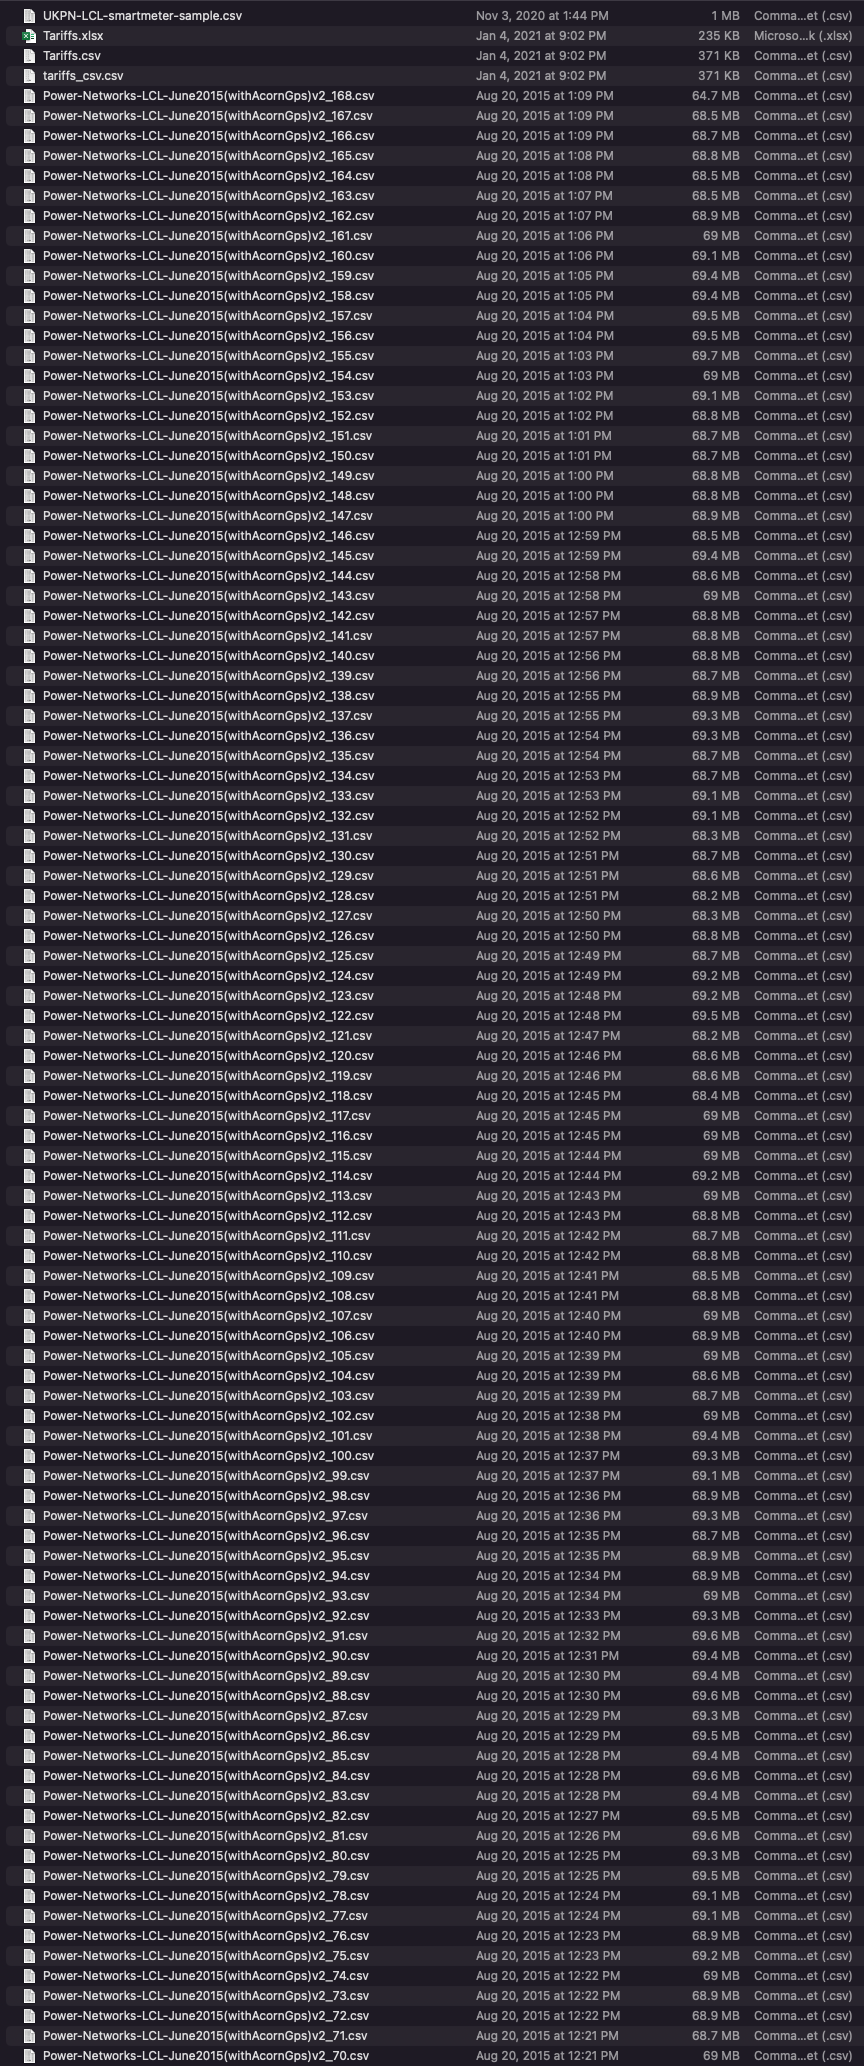
\includegraphics[width=0.95\textwidth]{images/lcl-raw-files.png}
\end{frame}

\begin{frame}{Data Prep, Cleaning, Processing}
  \begin{enumerate}
    \item<+-> first set of files, segmented by year, contain the \texttt{house\_id} (str), \texttt{treated} (bool), \texttt{date\_time} (datetime), \texttt{KWH/hh} (float).
    \item<+-> second contains \texttt{house\_id} (str), \texttt{acorn} (str), \texttt{acorn\_group} (str).
    \item<+-> third is the tarrif file contains \texttt{date\_time} (datetime), price per designation for that hh (float).
  \end{enumerate}
\end{frame}

\begin{frame}{Data Prep, Cleaning, Processing}
  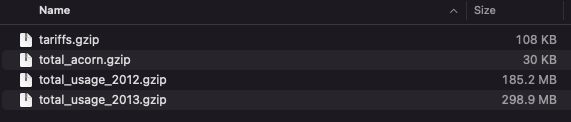
\includegraphics[width=0.95\textwidth]{images/lcl-clean-files.png}
\end{frame}

\begin{frame}{Our matrics are half full for 2012}
  \begin{multicols}{2}
    $$
    \alpha_{2012} = \left[\begin{array}{cccc}
    a_{11} & a_{12} & \cdots & a_{1 n_c} \\
    a_{21} & a_{22} & \cdots & a_{2 n_c} \\
    \vdots & \vdots & \ddots & \vdots \\
    a_{t 1} & a_{t 2} & \cdots & a_{t n_c}
    \end{array}\right]
    $$
    \break
    \centering
    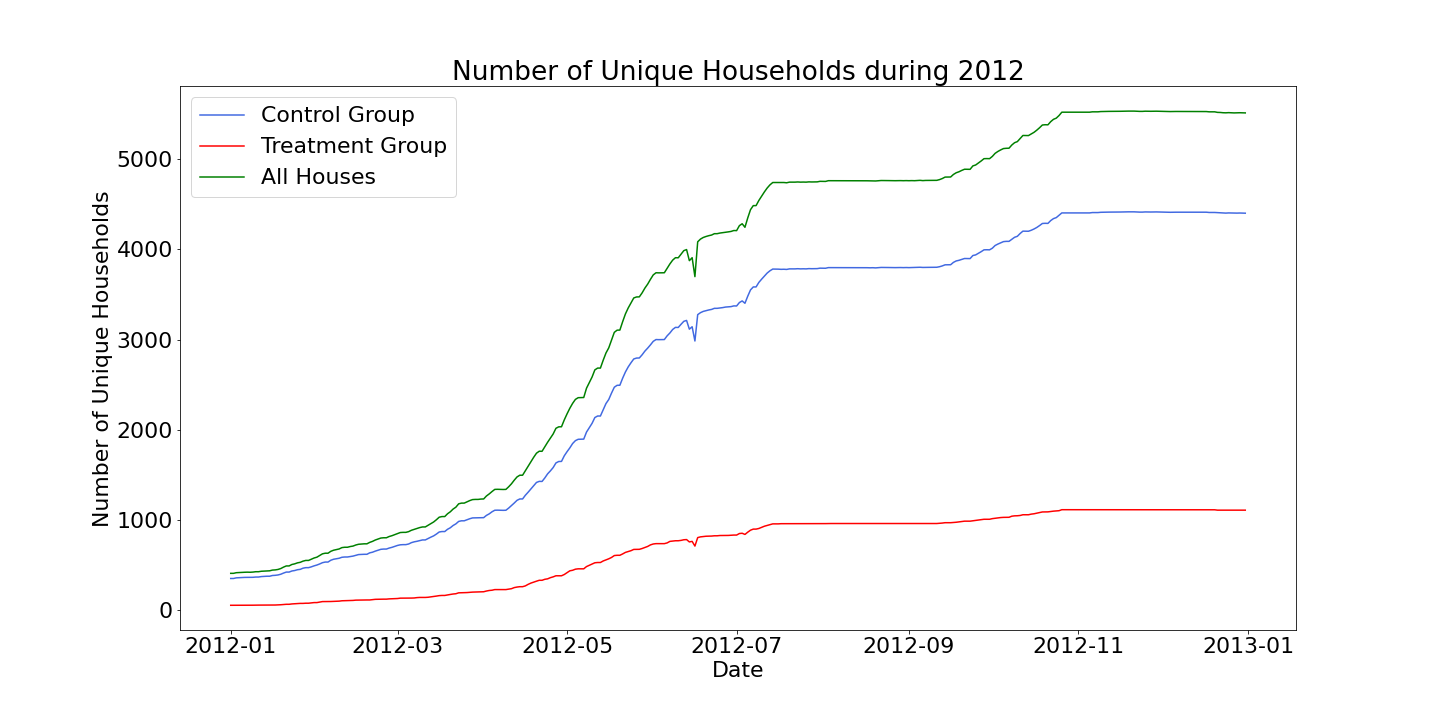
\includegraphics[width=0.6\textwidth]{images/unique-houses-2012.png}
  \end{multicols}
  \vspace{-1cm}
  \begin{align*}
    \begin{split}
        \alpha_{2012} X &= \beta_{2012} \\
        \alpha_{2013} X &= \hat\beta_{2013} \\
        \Delta\mbox{treatment} &= \beta_{2013} - \hat\beta_{2013}
    \end{split}
  \end{align*}
  Our 2012 matrics are half full.
\end{frame}

\begin{frame}{We have some paths forward}
  \begin{itemize}
    \item<+-> impute values
    \begin{itemize}
      \item<+-> {\color{green}{pro}}: you are keeping all of your data and you can capture the full trend.
      \item<+-> how do you impute values?
      \item<+-> are you introducing error?
    \end{itemize}
  \end{itemize}
\end{frame}

\begin{frame}{We have some paths forward}
  \begin{itemize}
    \item<+-> limit the timeframe to, for example, latter half of 2012
    \begin{itemize}
      \item<+-> {\color{red}{con}}: can't capture annual seasonality
    \end{itemize}
  \end{itemize}
\end{frame}

\begin{frame}{We have some paths forward}
  \begin{itemize}
    \item<+-> use a fixed panel: only keep the houses that have values for all of 2012
    \begin{itemize}
      \item<+-> {\color{red}{con}}: you are making your sample size small
    \end{itemize}
  \end{itemize}
\end{frame}

\begin{frame}{We have some paths forward}
  \begin{itemize}
    \item<+-> reduce dimenstionality
    \begin{itemize}
      \item<+-> go from matrix of $t \times n$ to vector of size $t$.
      \item<+-> take the mean over all houses that you have at any given $t$ to remove this issue.
      \item<+-> {\color{red}{con}}: you are reducing dimenstionality and removing valuable datapoints that might teach you something
    \end{itemize}
  \end{itemize}
\end{frame}

\begin{frame}{The path forward depends on your usecase.}
  \begin{itemize}
    \item[]<+-> There is no wrong answer here. 
    \item[]<+-> The choice of methodology depends on the assumptions you are comfortable making.
    \item[]<+-> It's important to make informed decisions grounded in the type of analysis and with full knowledge of your data and its shortfalls.
  \end{itemize}
\end{frame}

% \begin{frame}{Other Clustering?}
%   I used different clustering methods to cluster houses in this data set based on the control group’s consumption pre-intervention: k-means clustering, PCA3, TSNE4. I also tried clustering on the frequency responses which I found fast Fourier trans- form. PCA, TSNE, and Agglomerative clustering on the resulting data set was also inconclusive. This is reason for sticking to the pre-existing socio-economic clusters.
% \end{frame}

\begin{frame}{Matrices $\rightarrow$ Vectors}
  \begin{multicols}{2}
    $$
    \alpha_y = \left[\begin{array}{cccc}
    a_{11} & a_{12} & \cdots & a_{1 n_c} \\
    a_{21} & a_{22} & \cdots & a_{2 n_c} \\
    \vdots & \vdots & \ddots & \vdots \\
    a_{t 1} & a_{t 2} & \cdots & a_{t n_c}
    \end{array}\right]
    \qquad\longrightarrow
    $$
    \break
    $$
    \overline{\alpha_y} = \left[\begin{array}{cccc}
    \overline{a_{1}} \\
    \overline{a_{2}} \\
    \vdots \\
    \overline{a_{t}}
    \end{array}\right]
    $$
  \end{multicols}
  where $\overline{a_{i}}$ = $\frac{\Sigma{a_{i, m}}}{n}$ where $a_{i, m}$ has a value and $n$ is the total number of elements with a value.
\end{frame}

\begin{frame}{Reduce dimenstionality}
  \begin{align*}
    \begin{split}
      \overline{\beta_{2012}} &= a \times \overline{\alpha_{2012}} + b \\
      \overline{\hat{\beta}_{2013}} &= a \times \overline{\alpha_{2013}} + b \\
      \overline{\Delta\mbox{treatment}} &= \overline{\beta_{2013}} - \overline{\hat{\beta}_{2013}}
    \end{split}
  \end{align*}
\end{frame}

\begin{frame}{Learned linear relationship from 2012}
  \centering
  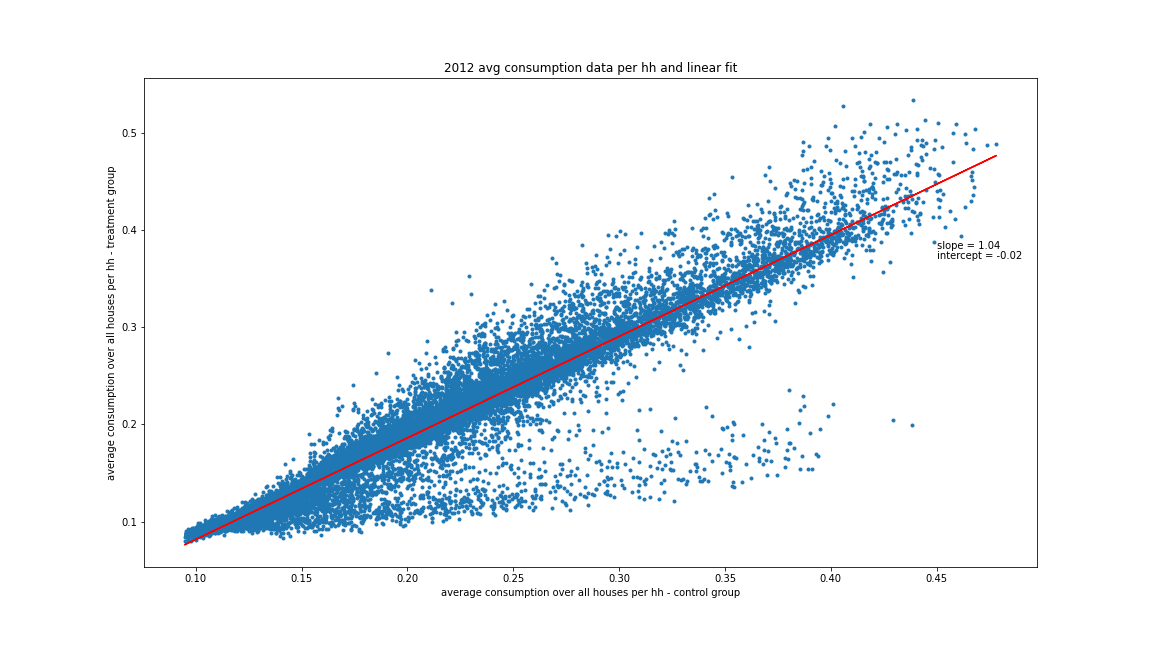
\includegraphics[width=1\textwidth]{images/2012-avg.png}
\end{frame}

\begin{frame}{Interpret the estimated treatment effect}
    $$
    \overline{T} = \left[\begin{array}{cccc}
    \overline{t_{1}} \\
    \overline{t_{2}} \\
    \overline{t_{3}} \\
    \overline{t_{4}} \\
    \vdots \\
    \overline{t_{i}} \\
    \overline{t_{i+1}} \\
    \vdots \\
    \overline{t_{t-1}} \\
    \overline{t_{t}}
    \end{array}\right]
    $$
\end{frame}

\begin{frame}{Interpret the estimated treatment effect}
  \centering
  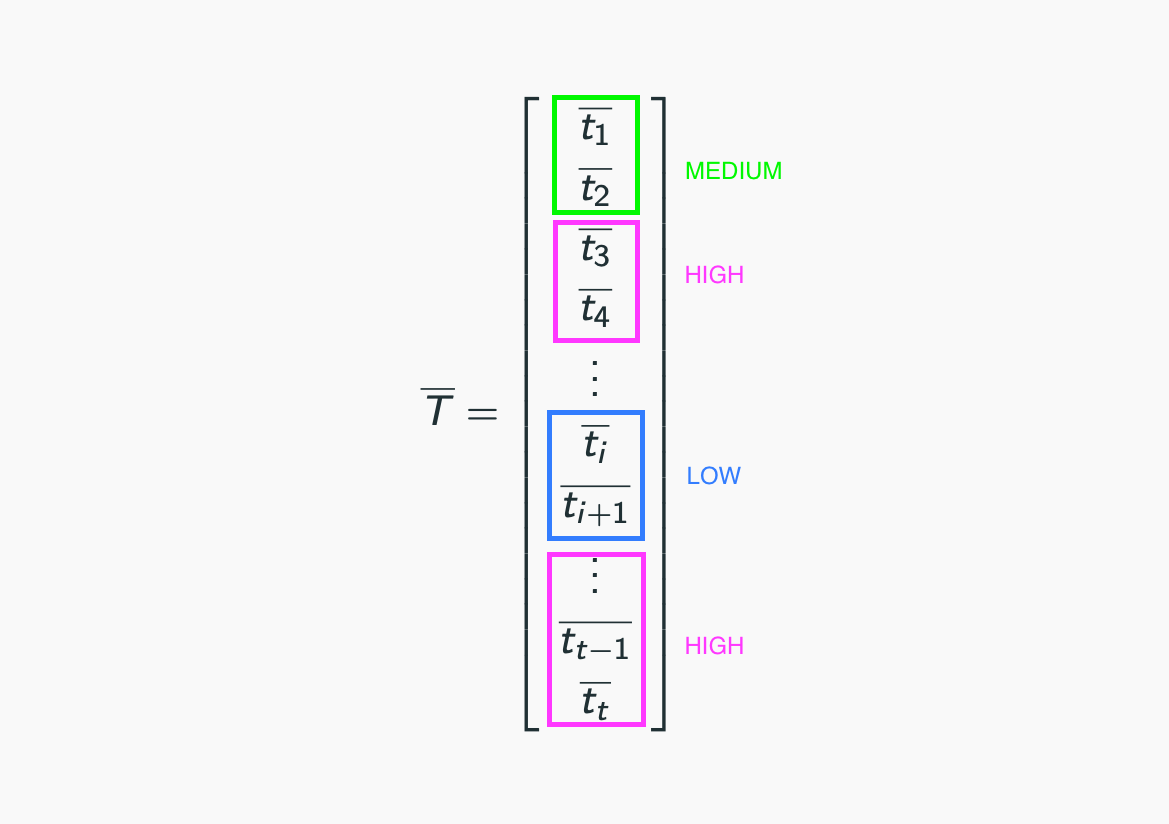
\includegraphics[width=1\textwidth]{images/linear-treatment-hours.png}
\end{frame}

\begin{frame}{Results}
  \centering
  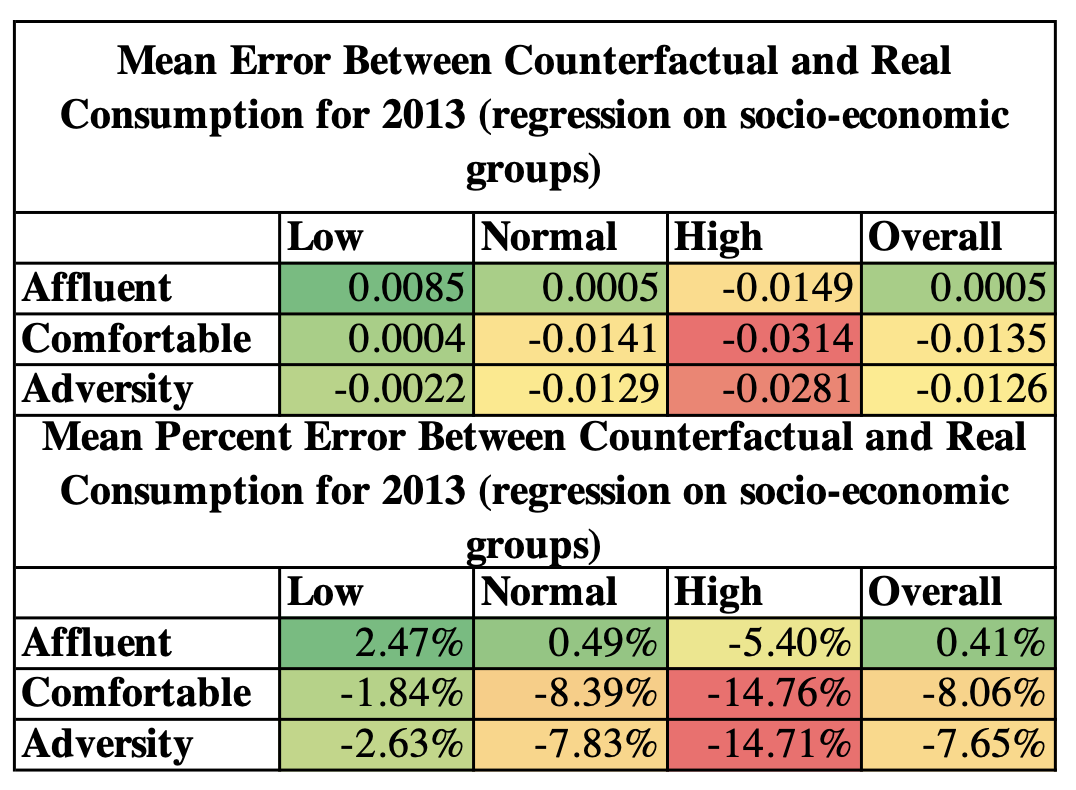
\includegraphics[width=1\textwidth]{images/agg-linreg-consumption2.png}
\end{frame}

\section{The Conclusion}

\begin{frame}{What Did We Learn?}
  \begin{itemize}
    \item<+-> A little bit about electricity markets.
    \item<+-> Causal analysis.
    \item<+-> How to break down your data to match the mathematical model at hand.
    \item<+-> Questions to ask before analysis:
    \begin{itemize}
      \item<+-> How was the data collected? 
      \item<+-> What biases are present?
      \item<+-> How does that impact your analysis and results?
    \end{itemize}
  \end{itemize}
\end{frame}

\begin{frame}{Takeaways}
  \begin{itemize}
    \item<+-> KYD: know your data: learn how it was collected, its biases, shortcomings, feature space, problem space.
    \item<+-> Before diving into fitting a model to your data, it's important to base your analysis on some mathematical model
    \vspace{1cm}
    \begin{center}
    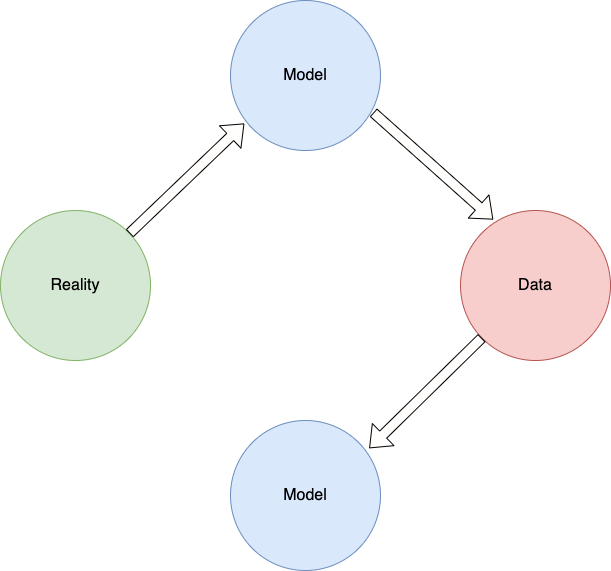
\includegraphics[width=0.8\textwidth]{images/reality-model-data.png}
    \end{center}
  \end{itemize}
\end{frame}

\begin{frame}{Thank You! Questions?}
  \begin{itemize}
  \item \url{https://github.com/sabanejad}
  \item \url{https://www.linkedin.com/in/sabanejad/}
  \item \url{https://dspace.mit.edu/handle/1721.1/144969}
  \end{itemize}
\end{frame}

% \section{Appendix}

% \begin{frame}{Who are System Operators?}
%   \item<+-> \textbf{System Operators}: Resposible for reliable delivery of electricity to consumers.
%   \vspace{0.2cm}
%   \begin{center}
%     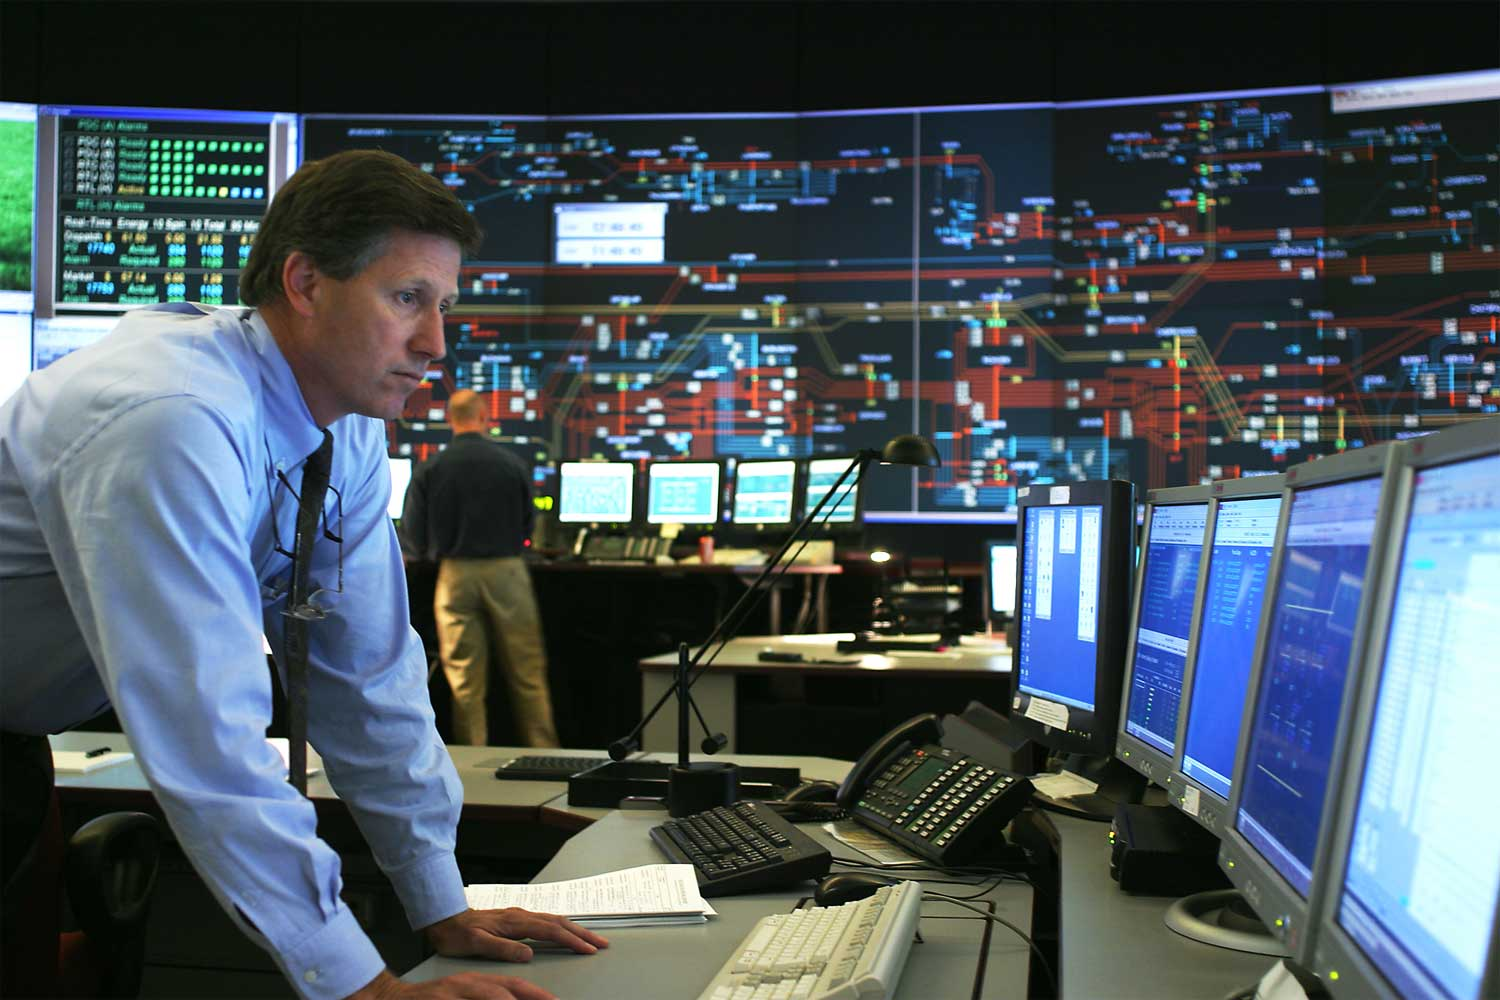
\includegraphics[width=0.65\textwidth]{images/iso-control-room.png}
%   \end{center}
% \end{frame}

% \begin{frame}{Socio DoW Analysis}
%   \centering
%   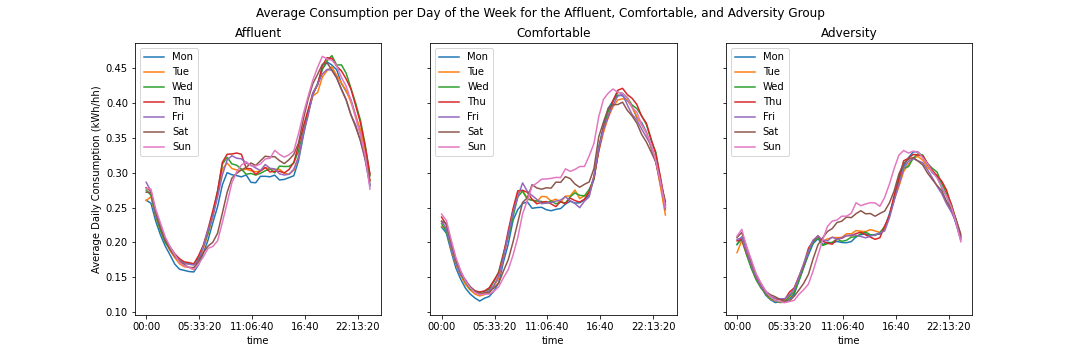
\includegraphics[width=1.1\textwidth]{images/dow-socio.png}
% \end{frame}

% \begin{frame}{Treatment vs Control Group Baselines}
%   $$
%   \begin{aligned}
%     & f_{2012}\left(\theta_{t r}, T, t\right) \quad \stackrel{h(t)}{\longrightarrow} \quad f_{2013}^*\left(\theta_{t r}, T, t\right) \\
%     & g\left(\theta_c\right) \uparrow \quad \quad \quad \quad \quad \quad g\left(\theta_c\right) \uparrow \\
%     & f_{2012}\left(\theta_c, T, t\right) \quad \stackrel{h(t)}{\longrightarrow} \quad f_{2013}\left(\theta_c, T, t\right) \\
%     &
%   \end{aligned}
%   $$
% \end{frame}

% \begin{frame}{The Fundamental Problem of Causal Inference (FPCI)}
%   \begin{itemize}
%     \item<+-> Assume $X \in\{0,1\}$ is a binary causal variable and $Y$ is a response variable (which may be continuous).
%     \item<+-> Assume $X$ has a causal effect on $Y$, this implies that the value of $Y$ we observe depends on the value of $X$.
%     \item<+-> We can define $Y_0$ and $Y_1$ as the values that $Y$ would take if $X$ were equal to 0 and 1 respectively.
%     \item<+-> $Y_0$ and $Y_1$ are counterfactuals of one another. Both can never be observed at the same time.
%     \begin{itemize}
%       \item $Y_i$ := the outcome of interest for unit $i$
%       \item $Y_0$ := the value of $Y_i$ for $X=0$ (untreated unit)
%       \item $Y_1$ := the value of $Y_i$ for $X=1$ (treated unit)
%     \end{itemize}
%   \end{itemize}
% \end{frame}

% \begin{frame}{The Fundamental Problem of Causal Inference (FPCI)}
%   \begin{itemize}
%     \item<+-> Assume that units are all alike, so $Y_{0 i} \equiv Y_0$ and $Y_{1 i} \equiv Y_1$.
%     \item<+-> The causal effect of $X_i$ on $Y_i$ is $T=Y_1-Y_0$, where $T$ stands for Treatment Effect.
%     \item<+-> \textit{But what's the issue here?}
%     \item<+-> We never observe $Y_1-Y_0$ for a single unit $i$. Instead, we observe
%     $$
%     Y_i=Y_{1 i} X_i+Y_{0 i}\left(1-X_i\right)
%     $$
%     That is, we observe $Y_1$ or $Y_0$ but not both.
%   \end{itemize}
% \end{frame}

% \begin{frame}{Estimate Causal Effects for Populations Rather than Units}
%   \begin{itemize}
%     \item<+-> Causal Effect for Unit $i$: $T_i=Y_{1 i}-Y_{0 i}$
%     \begin{itemize}
%       \item \textit{We can't estimate this. Why?}
%     \end{itemize}
%     \item<+-> Average Treatment Effect for the Treated (ATT): $T^*=E\left[Y_1-Y_0 \mid X=1\right]$
%     \item<+-> Average Treatment Effect (ATE): $T^{\dagger}=E\left[Y_1-Y_0\right]$
%     \item<+-> \textit{ATE is treatment effect assuming entire population is treated.}
%       \begin{itemize}
%         \item \textit{What's an example?}
%         \item \textit{Which of the two is more important? But how do we estimate it?}
%       \end{itemize}
%   \end{itemize}
% \end{frame}

% \begin{frame}{Estimate Causal Effects for Populations Rather than Units}
%   To make things more complicated, let's make another estimator.
%   \begin{enumerate}
%     \item<+-> $\tilde{T}=E[Y \mid X=1]-$ $E[Y \mid X=0]$
%   \end{enumerate}
%   Is $\tilde{T}$ a good estimator of $T^*$? What is it estimating?
%   What change can we make to our population to make this a good estimator?
% \end{frame}

% \begin{frame}{Estimate Causal Effects for Populations Rather than Units}
%   \begin{itemize}
%     \item<+-> Assume your treatment and control group had the same expected baseline behavior, and the same counterfactual expected behavior.
%     $$
%     \begin{aligned}
%     & E\left[Y_1 \mid X=1\right]=E\left[Y_1 \mid X=0\right] \\
%     & E\left[Y_0 \mid X=1\right]=E\left[Y_0 \mid X=0\right]
%     \end{aligned}
%     $$
%     \item<+-> Let's revisit $$ \begin{aligned}
%       T^* & = E\left[Y_1 \mid X=1\right]-E\left[Y_0 \mid X=1\right] \\
%           & = E\left[Y_1 \mid X=1\right]-E\left[Y_0 \mid X=0\right] 
%     \end{aligned} $$
%   \end{itemize}
% \end{frame}

% \begin{frame}{Estimate Causal Effects for Populations Rather than Units}
%   \begin{itemize}
%     \item<+-> but what if they aren't exactly the same, this would often hold in the case of an actual treatment. In other words there's a reason for the treatment:
%     \item<+-> $$
%     \begin{aligned}
%     & E\left[Y_1 \mid X=1\right]>E\left[Y_1 \mid X=0\right] \\
%     & E\left[Y_0 \mid X=1\right]>E\left[Y_0 \mid X=0\right] .
%     \end{aligned}
%     $$
%     \item<+-> ... let's bring back $\tilde{T}$. 
%   \end{itemize}
% \end{frame}

% \begin{frame}{Estimate Causal Effects for Populations Rather than Units}
%   So, if we calculated the contrast $\tilde{T}=E[Y \mid X=1]-E[Y \mid X=0]$ for this unbalanced group, what would we get?
%   $$
%   \begin{aligned}
%   E\left[Y_1 \mid X=1\right]-E\left[Y_0 \mid X=0\right] & =\underbrace{E\left[Y_1 \mid X=1\right]-E\left[Y_0 \mid X=1\right]}_{T^*} \\
%   & +\underbrace{\left\{E\left[Y_0 \mid X=1\right]-E\left[Y_0 \mid X=0\right]\right\}}_{\text {Bias }} .
%   \end{aligned}
%   $$
%   (Go to whiteboard and do the rest)
% \end{frame}

% % Notice that our substitution above of $E\left[Y_0 \mid X=1\right]$ for $E\left[Y_0 \mid X=0\right]$ is justified by the assumption of treatment-control balance in equation (1). If the subjects who didn't receive the treatment are just like those who did but for not having received the treatment, then the contrast between the treated and untreated groups provides an unbiased estimate of the causal effect of the treatment on the treated group (ATT).
% % - Returning to our invalid estimator $\tilde{T}$, let's ask how likely is it that the counterfactual outcomes would be balanced among a set of people selected from the population according to whether or not they are currently receiving the treatment. It does not take a great leap of logic to hypothesize that the patients receiving the cholesterol drug are more likely to be suffering from high cholesterol than those who are not taking the drug. This would imply that:


% % In words, patients receiving the drug are more likely to suffer from high cholesterol whether or not they are receiving the drug (presumably, they are receiving the drug specifically because they were diagnosed with high cholesterol).


% % The first term on the right-hand side of this equation is the true, causal effect of the cholesterol treatment on those who take it (the ATT). The second term is the potential bias that


% \begin{frame}{Potential Outcomes Framework (Rubin-Neyman Causal Model)}
%   Each household $x_i$ has two potential outcomes:
%   \begin{itemize}
%     \item $Y_0\left(x_i\right)$ is the potential outcome had the unit not been treated (static pricing model): ``control outcome"
%     \item $Y_1\left(x_i\right)$ is the potential outcome had the unit been treated (dToU pricing model): ``treated outcome"
%   \end{itemize}
%   - Conditional average treatment effect for unit $i$ :
%   $$
%   \operatorname{CATE}\left(x_i\right)=\mathbb{E}_{Y_1 \sim p\left(Y_1 \mid x_i\right)}\left[Y_1 \mid x_i\right]-\mathbb{E}_{Y_0 \sim p\left(Y_0 \mid x_i\right)}\left[Y_0 \mid x_i\right]
%   $$
%   - Average Treatment Effect:
%   $$
%   A T E:=\mathbb{E}\left[Y_1-Y_0\right]=\mathbb{E}_{x \sim p(x)}[\operatorname{CATE}(x)]
%   $$
% \end{frame}

% \begin{frame}{Mathematical Model}
% \begin{itemize}
%   \item Fundamental Problem of Causal Inference: Both outcomes can't be observed for the same household $x_i$.
%   \begin{itemize}
%     \item Observed factual outcome:
%     $$
%     y_i=t_i Y_1\left(x_i\right)+\left(1-t_i\right) Y_0\left(x_i\right)
%     $$
%     \item Unobserved counterfactual outcome:
%     $$
%     y_i^{C F}=\left(1-t_i\right) Y_1\left(x_i\right)+t_i Y_0\left(x_i\right)
%     $$
%   \end{itemize}
%   \item Solution? Approximate the counterfactual eg close enough to random sample: minimum wage problem, NJ and east PA, Card \& Krueger, 1994.
% \end{itemize}
% \end{frame}

% \begin{frame}
%   David Card minimum wage paper: \url{https://davidcard.berkeley.edu/papers/njmin-aer.pdf}
%   LCL Experiment \url{https://data.london.gov.uk/dataset/smartmeter-energy-use-data-in-london-households}
% \end{frame}

\end{document}